\subsubsection{Overview}

The Sequencer is a critical off-chain component of the ZK-Rollup responsible for collecting, validating, ordering, and batching user transactions before they are processed by the Executor. Implemented in Rust for performance and memory safety, the Sequencer acts as the primary interface between end-users and the rollup's execution layer, while also maintaining synchronization with Layer 1 (L1) Ethereum to handle priority operations. By handling the complexity of transaction ordering and validation off-chain, the Sequencer enables the high throughput and low latency characteristic of rollups, deferring the computationally expensive proof generation to the Executor.

\subsubsection{Architectural Components}

\begin{figure}[htbp]
 \begin{adjustwidth}{0cm}{}
  \centering
  \includegraphics[height=0.95\linewidth, angle=0]{figures/sequencer.png}
  \caption{Sequencer architecture.}
  \label{fig:operation-flow}
 \end{adjustwidth}
\end{figure}

The sequencer is implemented as a modular Rust crate, organized into clearly separated components. Several well-known design patterns---including Strategy, Factory Method, Composition Root, Shared State, Observer, and Pipeline---are applied throughout the implementation to achieve extensibility and maintainability. Each pattern is discussed in context within the component that employs it.

\subsubsubsection{Sequencer API (JSON-RPC Endpoint)}

The Sequencer API serves as the public gateway for all user interactions with the rollup. By exposing a JSON-RPC interface compatible with standard Ethereum wallet clients, it allows users to submit signed transactions using familiar tooling (e.g., MetaMask, ethers.js) without needing specialized software.

The application startup follows the \textbf{Composition Root} pattern: the \texttt{main.rs} entry point creates all shared resources (state cache, transaction pools) at the top level and distributes them to components via \texttt{Arc} references, wiring three concurrent async tasks---the API server, the L1 listener, and the batch orchestrator:

\begin{lstlisting}[style=rustStyle, caption={Composition root wiring components}, label={lst:main}]
let state_cache = StateCache::new();
let tx_pool = Arc::new(TransactionPool::new());
let forced_queue = Arc::new(ForcedQueue::new());

// L1 listener and batch orchestrator run as background tasks
tokio::spawn(async move { l1_listener.start().await; });
tokio::spawn(async move { orchestrator.start().await; });

// API server blocks on main thread
server.start().await
\end{lstlisting}

The API itself is implemented using the \textbf{Axum} web framework with Tokio as the async runtime. Incoming JSON-RPC requests are routed to handlers based on the method name. The \texttt{sendTransaction} handler orchestrates the full transaction lifecycle---deserialization, validation, pool insertion, and soft confirmation:

\begin{lstlisting}[style=rustStyle, caption={Transaction submission handler}, label={lst:send-tx}]
async fn handle_send_transaction(state: AppState, request: JsonRpcRequest)
    -> Json<JsonRpcResponse>
{
    let tx: UserTransaction = serde_json::from_value(request.params.clone())?;
    match state.validator.validate(&tx).await {
        Ok(()) => {
            state.state_cache.increment_nonce(&tx.from).await;
            state.tx_pool.add(tx.clone()).await;
            // Return SoftConfirmation with Accepted status
        }
        Err(validation_error) => {
            // Return SoftConfirmation with Rejected { reason } status
        }
    }
}
\end{lstlisting}

\subsubsubsection{Validity Checker}

Before entering the transaction pool, all submitted transactions must pass through a rigorous multi-stage validation pipeline to ensure network integrity and prevent spam. The \texttt{Validator} performs three sequential checks against the state cache:

\begin{lstlisting}[style=rustStyle, caption={Three-stage validation pipeline}, label={lst:validator}]
pub async fn validate(&self, tx: &UserTransaction)
    -> Result<(), ValidationError>
{
    self.verify_signature(tx)?;    // ECDSA signature recovery
    self.check_nonce(tx).await?;   // Sequential nonce enforcement
    self.check_balance(tx).await?; // Sufficient funds for value + gas
    Ok(())
}
\end{lstlisting}

\paragraph{Signature Verification}
The checker uses ECDSA signature recovery to verify that the transaction was signed by the claimed sender. The recovered address is compared against the \texttt{from} field---a mismatch indicates forgery.

\paragraph{Nonce Validation}
Each transaction's nonce must exactly match the account's current nonce, enforcing strict sequential ordering and preventing replay attacks.

\paragraph{Balance Verification}
The checker confirms the sender has sufficient funds to cover both the transfer value and gas fees (\texttt{gas\_price} $\times$ \texttt{gas\_limit}), filtering out invalid transactions early.

\subsubsubsection{Local State Cache}

To achieve high throughput, the Sequencer relies on the Local State Cache, an in-memory key-value store that maintains a fast-access replica of the current rollup state. The cache applies the \textbf{Shared State} pattern: it is implemented using a \texttt{HashMap<Address, AccountState>} protected by Tokio's asynchronous \texttt{RwLock} and wrapped in \texttt{Arc}, enabling concurrent read access during validation with exclusive writes for nonce updates. This same pattern is applied to the transaction pool and forced queue, allowing all concurrent components to safely share data.

A key design choice is the \texttt{get\_or\_init\_account} method, which returns default values (zero balance, nonce 0) for unknown accounts \emph{without} inserting them into the cache, preventing memory inflation from validation attempts against non-existent accounts.

This cache is periodically synchronized with updates from the State Manager component in the Executor, implementing an eventually-consistent model that accepts brief staleness in exchange for sub-millisecond read latencies during validation.

\subsubsubsection{Transaction Pool}

Valid normal (non-priority) transactions are held in the Transaction Pool, implemented as a FIFO queue using Rust's \texttt{VecDeque} for efficient $O(1)$ insertion and removal. The \texttt{get\_pending(max)} method atomically drains up to \texttt{max} transactions, ensuring each transaction is consumed exactly once by the batch production pipeline.

\subsubsubsection{L1 Event Listener}

The L1 Event Listener follows the \textbf{Observer} pattern: it subscribes to blockchain events from the RollupBridge smart contract on Ethereum L1 and reacts to deposit and forced-exit notifications by populating the forced transaction queue. It uses the \texttt{ethers-rs} library's \texttt{abigen!} macro to create type-safe event filters directly from Solidity event signatures, and connects via WebSocket for real-time event streaming.

The listener uses Tokio's \texttt{select!} macro to concurrently process both Deposit and ForcedExit event streams. Each detected event is parsed into a \texttt{ForcedTransaction} and added to the forced queue. The listener implements an automatic reconnection loop with block checkpoint tracking, maintaining an at-least-once delivery guarantee---if the WebSocket connection drops, it resumes from the last processed block after a configurable retry delay.

\subsubsubsection{Forced Transaction Queue}

Forced transactions originating from L1 events are placed in a dedicated priority queue, separate from the normal transaction pool. This design enforces a critical security property: \textbf{forced transactions are unskippable}. The \texttt{get\_all()} method atomically drains the entire queue, and the batch orchestrator must include all returned transactions in the next batch, preventing censorship and ensuring users can always exit the rollup even if the sequencer becomes malicious or unresponsive.

The forced queue implements strict FIFO ordering based on the order in which L1 events are received (corresponding to L1 block number and transaction index), ensuring deterministic processing order that can be verified by anyone monitoring the L1 chain.

\subsubsubsection{Scheduler (Policy Engine)}
\label{sec:scheduler}

The Scheduler implements the \textbf{Strategy design pattern} \cite{gamma1994design}, allowing the transaction ordering algorithm to be selected at runtime through configuration. The pattern decouples the scheduling context from the concrete ordering implementations through a trait interface:

\begin{figure}[htbp]
\centering
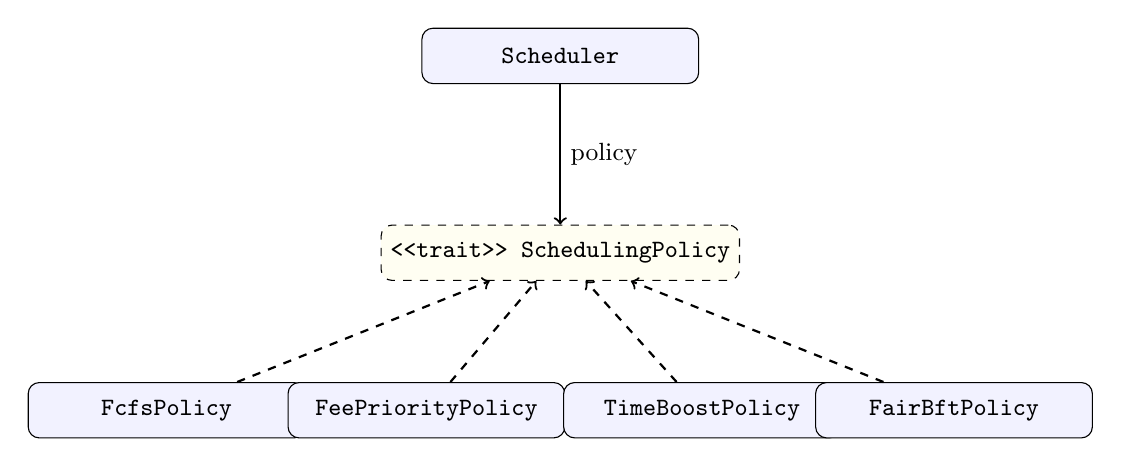
\begin{tikzpicture}[
    class/.style={rectangle, draw=black, rounded corners, minimum height=2em, minimum width=10em, font=\ttfamily\small, fill=blue!5},
    interface/.style={rectangle, draw=black, rounded corners, dashed, minimum height=2em, minimum width=10em, font=\ttfamily\small, fill=yellow!5},
    arrow/.style={->, thick},
    impl/.style={->, thick, dashed},
]
    % Interface
    \node[interface] (trait) at (0, 0) {<<trait>> SchedulingPolicy};
    
    % Context
    \node[class] (scheduler) at (0, 2.5) {Scheduler};
    
    % Concrete strategies
    \node[class] (fcfs) at (-5, -2) {FcfsPolicy};
    \node[class] (fee) at (-1.7, -2) {FeePriorityPolicy};
    \node[class] (tb) at (1.8, -2) {TimeBoostPolicy};
    \node[class] (bft) at (5, -2) {FairBftPolicy};
    
    % Relationships
    \draw[arrow] (scheduler) -- node[right, font=\small] {policy} (trait);
    \draw[impl] (fcfs) -- (trait);
    \draw[impl] (fee) -- (trait);
    \draw[impl] (tb) -- (trait);
    \draw[impl] (bft) -- (trait);
\end{tikzpicture}
\caption{Strategy design pattern applied to scheduling policies.}
\label{fig:strategy-pattern}
\end{figure}

The \texttt{SchedulingPolicy} trait defines the contract that all ordering strategies must implement. The \texttt{Scheduler} holds a boxed trait object (\texttt{Box<dyn SchedulingPolicy>}) for runtime polymorphism, and its \texttt{schedule()} method implements a two-phase ordering algorithm:

\begin{lstlisting}[style=rustStyle, caption={Strategy trait and scheduler context}, label={lst:scheduler}]
// Strategy interface
pub trait SchedulingPolicy: Send + Sync {
    fn order_transactions(&self, txs: Vec<UserTransaction>)
        -> Vec<UserTransaction>;
    fn name(&self) -> &str;
}

// Context: holds a strategy and applies two-phase ordering
pub struct Scheduler {
    policy: Box<dyn SchedulingPolicy>,  // Runtime-selected strategy
}

impl Scheduler {
    pub fn schedule(&self, forced: Vec<ForcedTransaction>,
                    normal: Vec<UserTransaction>) -> Vec<Transaction> {
        let mut result = Vec::new();
        // Phase 1: ALL forced transactions first (non-negotiable)
        for tx in forced { result.push(Transaction::Forced(tx)); }
        // Phase 2: Normal transactions ordered by selected policy
        for tx in self.policy.order_transactions(normal) {
            result.push(Transaction::Normal(tx));
        }
        result
    }
}
\end{lstlisting}

The scheduling policy is selected through the TOML configuration file, parsed into a \texttt{SchedulingPolicyType} enum, and instantiated via a \textbf{Factory Method} pattern. The \texttt{create\_policy()} function maps each enum variant to its concrete policy implementation, decoupling policy creation from usage:

\begin{lstlisting}[style=rustStyle, caption={Factory method for policy creation}, label={lst:factory}]
pub fn create_policy(policy_type: SchedulingPolicyType)
    -> Box<dyn SchedulingPolicy>
{
    match policy_type {
        SchedulingPolicyType::Fcfs => Box::new(FcfsPolicy),
        SchedulingPolicyType::FeePriority => Box::new(FeePriorityPolicy),
        SchedulingPolicyType::TimeBoost { time_window_ms } =>
            Box::new(TimeBoostPolicy { time_window_ms }),
        SchedulingPolicyType::FairBft => Box::new(FairBftPolicy),
    }
}
\end{lstlisting}

This enables runtime switching without code changes:

\begin{lstlisting}[language={}, caption={Switching scheduling policy via configuration}, label={lst:sched-config}]
[scheduling]
policy_type = "FCFS"        # Options: "FCFS", "FeePriority",
                            #          "TimeBoost", "FairBFT"
time_window_ms = 5000       # Only used for TimeBoost policy
\end{lstlisting}

Four concrete strategies are implemented, each encapsulating a distinct ordering algorithm:

\begin{itemize}
    \item \textbf{FCFS (First-Come-First-Served)}: Maintains the original submission order with $O(1)$ overhead---the simplest and most predictable policy.
    \item \textbf{Fee-Priority}: Sorts transactions by \texttt{gas\_price} in descending order ($O(n \log n)$), maximizing sequencer revenue but potentially starving low-fee transactions.
    \item \textbf{Time-Boost}: Divides time into configurable discrete windows (e.g., 5-second slots) and applies a multi-key sort within each window---first by \texttt{boost\_bid} (a premium bid field), then by \texttt{gas\_price}, then FCFS for tie-breaking. This provides predictable latency guarantees with granular fairness.
    \item \textbf{Fair BFT Ordering}: Sorts strictly by transaction timestamp (ascending) to provide time-based fairness and MEV resistance. The current implementation targets a single-node sequencer; a multi-node extension would add BFT consensus for canonical timestamp agreement.
\end{itemize}

As an example, the Fee-Priority strategy simply sorts by gas price, while the Time-Boost strategy uses a more complex multi-key comparator:

\begin{lstlisting}[style=rustStyle, caption={Concrete strategy implementations (Fee-Priority and Time-Boost)}, label={lst:policies}]
// Fee-Priority: highest gas price first
impl SchedulingPolicy for FeePriorityPolicy {
    fn order_transactions(&self, mut txs: Vec<UserTransaction>)
        -> Vec<UserTransaction> {
        txs.sort_by(|a, b| b.gas_price.cmp(&a.gas_price));
        txs
    }
}

// Time-Boost: windowed ordering with premium bids
impl SchedulingPolicy for TimeBoostPolicy {
    fn order_transactions(&self, mut txs: Vec<UserTransaction>)
        -> Vec<UserTransaction> {
        txs.sort_by(|a, b| {
            let window_a = a.timestamp / self.time_window_ms;
            let window_b = b.timestamp / self.time_window_ms;
            match window_a.cmp(&window_b) {
                Ordering::Equal => {
                    let boost_a = a.boost_bid.unwrap_or_default();
                    let boost_b = b.boost_bid.unwrap_or_default();
                    match boost_b.cmp(&boost_a) {
                        Ordering::Equal => b.gas_price.cmp(&a.gas_price),
                        other => other,
                    }
                }
                other => other,
            }
        });
        txs
    }
}
\end{lstlisting}

This Strategy-based architecture satisfies the Open/Closed Principle: new ordering policies can be added by implementing the \texttt{SchedulingPolicy} trait without modifying the existing scheduler or orchestrator code, and different policies can be benchmarked under identical workloads by changing a single configuration value.

\subsubsubsection{Batch Engine}

The Batch Engine aggregates ordered transactions into sealed batches ready for execution. It maintains a monotonically increasing batch ID counter and enforces gas limits by tracking cumulative gas consumption as transactions are added:

\begin{lstlisting}[style=rustStyle, caption={Gas limit enforcement in batch engine}, label={lst:gas-limit}]
pub fn can_add_transaction(&self, current_txs: &[Transaction],
                            new_tx: &Transaction) -> bool {
    let current_gas: u64 = current_txs.iter()
        .map(|tx| tx.gas_limit()).sum();
    let total_gas = current_gas.saturating_add(new_tx.gas_limit());
    total_gas <= self.config.max_gas_limit
}
\end{lstlisting}

This check ensures no batch exceeds the configured gas limit that would make L1 verification prohibitively expensive. The \texttt{saturating\_add} prevents integer overflow during gas accumulation.

\subsubsubsection{Batch Orchestrator}

The Batch Orchestrator implements the \textbf{Pipeline} pattern, coordinating a multi-stage batch production flow: transactions move from Queue $\rightarrow$ Scheduler $\rightarrow$ BatchEngine $\rightarrow$ sealed Batch. It connects the forced queue, transaction pool, scheduler, and batch engine, running as a background async task with a dual-trigger batching mechanism:

\paragraph{Time-Based Trigger}
If the configured \texttt{timeout\_interval\_ms} expires before reaching the size threshold, the engine seals a partial batch to prevent unbounded latency during low-activity periods.

\paragraph{Size-Based Trigger}
When the number of queued transactions reaches the configured \texttt{max\_batch\_size}, a batch is immediately sealed.

The core \texttt{produce\_batch} method implements a four-step pipeline: (1) drain all forced transactions from the L1 queue, filtering by gas limit; (2) pull normal transactions from the pool, enforcing both size and gas limits; (3) combine both sets with forced transactions first; and (4) seal the batch via the \texttt{BatchEngine}.

\subsubsubsection{Batch Configuration}
\label{sec:batch-config}

The Sequencer's behavior is driven by a TOML configuration file loaded through Rust's \texttt{serde} deserialization framework. The configuration is organized into five sections, each mapping to a dedicated Rust struct:

\begin{lstlisting}[style=rustStyle, caption={Configuration structure hierarchy}, label={lst:config-structs}]
#[derive(Debug, Clone, Deserialize)]
pub struct Config {
    pub batch: BatchConfig,         // Batching parameters
    pub scheduling: SchedulingConfig, // Policy selection
    pub api: ApiConfig,             // JSON-RPC endpoint
    pub l1: L1Config,               // L1 connection settings
    pub database: DatabaseConfig,   // Registry storage
}
\end{lstlisting}

At startup, the configuration is loaded from a TOML file and used to initialize all components. The configuration flow works as follows: the \texttt{Config::load()} method reads and parses the TOML file, then each section is passed to its corresponding component. For example, the scheduling policy is resolved from the string-based TOML value (\texttt{"FCFS"}, \texttt{"FeePriority"}, etc.) into a \texttt{SchedulingPolicyType} enum, which the factory function (Listing~\ref{lst:factory}) uses to instantiate the correct strategy object:

\begin{lstlisting}[style=rustStyle, caption={Configuration to component wiring}, label={lst:config-wiring}]
let config = Config::load("config/default.toml")?;

// Scheduling policy: TOML string -> enum -> concrete strategy
let orchestrator = BatchOrchestrator::new(
    forced_queue.clone(),
    tx_pool.clone(),
    config.batch.clone(),                // BatchConfig -> engine
    config.scheduling.to_policy_type(),  // "FCFS" -> SchedulingPolicyType::Fcfs
);
\end{lstlisting}

The batch-specific parameters directly control the throughput-latency-cost trade-off. The default configuration demonstrates the tunable parameters:

\begin{lstlisting}[language={}, caption={Default sequencer configuration (\texttt{config/default.toml})}, label={lst:default-config}]
[batch]
max_batch_size = 100          # Max transactions per batch
timeout_interval_ms = 5000    # Seal partial batch after 5 seconds
min_batch_size = 10           # Minimum transactions before timeout seal
max_gas_limit = 30000000      # 30M gas limit per batch

[scheduling]
policy_type = "FCFS"          # Transaction ordering strategy

[api]
host = "127.0.0.1"
port = 3000

[l1]
rpc_url = "https://sepolia.infura.io/v3/YOUR_KEY"
bridge_address = "0x742d35Cc6634C0532925a3b844Bc9e7595f0bEb"
start_block = 18500000

[database]
url = "sqlite://sequencer.db"
\end{lstlisting}

These parameters directly influence system behavior:
\begin{itemize}
    \item \textbf{max\_batch\_size} and \textbf{timeout\_interval\_ms}: Larger batches and longer timeouts amortize fixed costs (proof generation, L1 submission) across more transactions, reducing per-transaction cost but increasing user-perceived latency. Smaller values improve responsiveness at the expense of higher overhead.
    \item \textbf{max\_gas\_limit}: Caps the computational cost per batch to ensure L1 proof verification remains economical. The batch engine uses the \texttt{can\_add\_transaction()} method (Listing~\ref{lst:gas-limit}) to enforce this limit iteratively as transactions are added.
    \item \textbf{policy\_type}: Selects the scheduling strategy at runtime (see Section~\ref{sec:scheduler}), enabling experimental comparison without recompilation.
\end{itemize}

The optimal configuration depends on network activity patterns and application requirements, which is why these parameters are exposed for experimental tuning in this research prototype.

\subsubsubsection{Batch Registry}

The Batch Registry is a persistent metadata store (backed by SQLite via the \texttt{sqlx} crate) that records the history of all produced batches. For each batch, it stores lightweight metadata: batch ID, transaction counts (total and forced), creation timestamp, and the scheduling policy used. This registry serves as an audit trail for verifiable sequencer decisions, enables crash recovery after restarts, and supports post-hoc analysis of batching efficiency and policy effectiveness during benchmarking.

\subsubsection{Operational Flow}

\begin{figure}[htbp]
 \begin{adjustwidth}{0cm}{}
  \centering
  \includegraphics[height=0.95\linewidth, angle=0]{figures/sequencer_pipeline.png}
  \caption{Sequencer flow.}
  \label{fig:sequencer-pipeline-flow}
 \end{adjustwidth}
\end{figure}

The complete sequencer workflow proceeds as follows:

\begin{enumerate}
    \item \textbf{User Transaction Submission}: A user submits a signed \texttt{UserTransaction} to the Sequencer API JSON-RPC endpoint via an HTTP POST request.
    
    \item \textbf{Validation}: The \texttt{Validator} performs three sequential checks against the \texttt{StateCache}: ECDSA signature verification, nonce validation, and balance sufficiency. Valid transactions receive a \texttt{SoftConfirmation} with \texttt{Accepted} status; invalid transactions are rejected immediately with a descriptive \texttt{ValidationError}.
    
    \item \textbf{Pool Insertion}: Valid transactions are inserted into the \texttt{TransactionPool} (FIFO queue), awaiting batch inclusion. The sender's nonce is immediately incremented in the \texttt{StateCache}.
    
    \item \textbf{L1 Event Monitoring}: Concurrently, the \texttt{L1Listener} streams \texttt{Deposit} and \texttt{ForcedExit} events from the RollupBridge contract via WebSocket and places corresponding \texttt{ForcedTransaction} instances into the \texttt{ForcedQueue}.
    
    \item \textbf{Scheduling}: When the \texttt{BatchOrchestrator} timer fires (controlled by \texttt{timeout\_interval\_ms}), the orchestrator pulls transactions from both queues and the \texttt{Scheduler} combines them:
    \begin{itemize}
        \item All pending forced transactions first (FIFO by L1 arrival order)
        \item Normal transactions ordered by the selected \texttt{SchedulingPolicy} (FCFS, FeePriority, TimeBoost, or FairBFT)
    \end{itemize}
    
    \item \textbf{Gas Limit Enforcement}: The orchestrator iteratively checks each transaction against the cumulative gas limit using \texttt{BatchEngine::can\_add\_transaction()}, stopping when the configured \texttt{max\_gas\_limit} is reached.
    
    \item \textbf{Batch Sealing}: The \texttt{BatchEngine} bundles the ordered transaction sequence, assigns a sequential Batch ID, records a UTC timestamp, and produces a sealed \texttt{Batch} ready for forwarding to the Executor component.
\end{enumerate}

\subsubsection{Design Rationale and Trade-offs}

\paragraph{Dual-Queue Architecture}

The separation of forced and normal transaction queues is a deliberate security design. By making forced transactions unskippable and always-first, the sequencer cannot censor user withdrawals even under malicious operation. This property is essential for maintaining the ``escape hatch'' that allows users to exit to L1 if the L2 becomes untrustworthy.

\paragraph{Configurable Scheduling Policies (Strategy Pattern)}

Different use cases demand different ordering guarantees. Financial applications may prioritize fee-based ordering to incentivize faster settlement, while gaming or social applications may prefer FCFS fairness. By applying the Strategy design pattern with a \texttt{SchedulingPolicy} trait and \texttt{Box<dyn SchedulingPolicy>} dynamic dispatch, the sequencer enables:

\begin{itemize}
    \item \textbf{Runtime configuration}: Switching policies via TOML without recompilation
    \item \textbf{Open/Closed Principle}: New policies are added by implementing the trait, without modifying existing code
    \item \textbf{Empirical comparison}: Different ordering rules can be benchmarked under identical workloads
\end{itemize}

\paragraph{Local State Cache vs. Authoritative State}

The Local State Cache trades strict consistency for performance. The \texttt{Arc<RwLock<HashMap>{>}{>}} design allows multiple concurrent readers (validation checks) with exclusive writers (nonce updates), enabling sub-millisecond read latencies. The cache accepts the risk of occasionally admitting transactions that will fail during execution (e.g., due to concurrent balance changes), relying on the Executor to enforce final correctness.

\paragraph{Async Concurrency Model}

The sequencer leverages Tokio's async runtime to run three concurrent components---the API server, L1 listener, and batch orchestrator---on a shared thread pool. Shared state is accessed through \texttt{Arc<RwLock<T>{>}{>}} wrappers, maximizing throughput on modern multi-core hardware without the overhead of inter-process communication.

\paragraph{Batch Size and Timeout Trade-offs}

The dual-trigger batching mechanism balances efficiency and responsiveness. The optimal configuration depends on network activity patterns and application requirements, which is why these parameters are exposed as TOML configuration for experimental tuning (see Section~\ref{sec:batch-config}).

\subsubsection{Integration with Other Components}

The Sequencer interfaces with:

\begin{itemize}
    \item \textbf{RollupBridge Contract (L1)}: Receives deposit and forced-exit events via WebSocket subscription using the \texttt{ethers-rs} library, generating priority forced transactions
    \item \textbf{Executor}: Forwards sealed \texttt{Batch} objects for state transition computation and proof generation
    \item \textbf{State Manager}: Receives state updates to keep the \texttt{StateCache} synchronized via the \texttt{update()} method
    \item \textbf{Users}: Provides the JSON-RPC API (via Axum) for transaction submission and soft confirmation responses
\end{itemize}

This modular design isolates sequencing logic from execution and proving, enabling independent optimization and replacement of components during benchmarking experiments.


This sequencer component forms the critical first stage of the ZK-Rollup pipeline, transforming a stream of user requests and L1 events into ordered, validated batches ready for cryptographic proof generation---bridging the gap between user experience and the mathematical guarantees provided by zero-knowledge proofs.

